
\section{Modelling}

In this section mathematical models of the UVMS is presented. The kinematics of the UVMS is highly complex due to the mix of quasi-velocities and generalized velocities, and the number of degrees of freedom of the total system. 
The dynamics is also highly complex, due to the high amount of parameters in the hydrodynamics, strong coupling forces between the rigid bodies, varying inertia for different manipulator configuration and more. The kinematics can be derived in the framework of Lie groups and Lie algebras. However, a detailed study of this is not included, but can be found in e.g. \cite{kristin_jant}. It should be noted that some of the notation is not consistent with the  litterature of underwater vehicles, due to the need to be consistent within the framework of the UVMS when refering to velocities. Instead of refering to the body velocity of the ship as $ \bs \nu$, the notation $ \vb{0b}{B}$ is used in order to comply with the notation used for velocities of the other frames in the UVMS. 
 

%kinematics
\subsection{Kinematics}

\begin{figure}[h!]
  \centering
  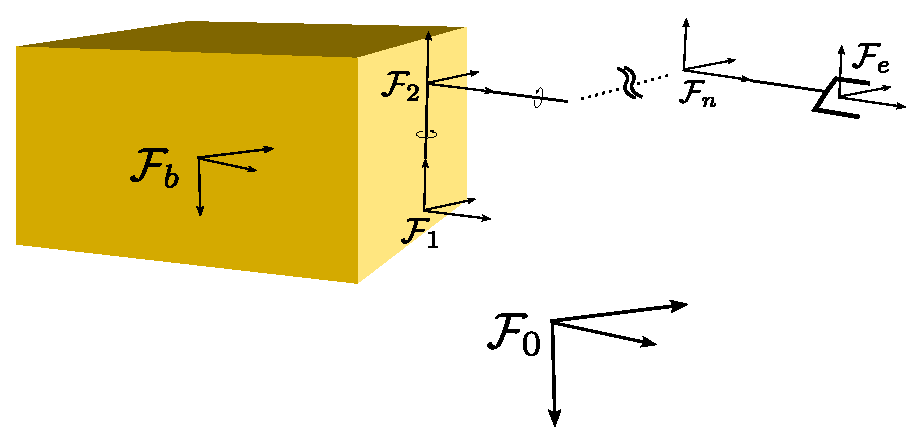
\includegraphics[scale=0.6]{./figures/uvms_kinematics.eps}
  \caption{The assignment of the frames for the UVMS system}
  \label{fig:uvms_kinematics}
\end{figure}
The ROV is regarded as a rigid body with the normal 6 degrees of freedom (DOFs), and the manipulator is a 6-link kinematic chain with only 1 DOF revolute joints. For representing the kinematic structure of the UVM system, a number of frames are assigned as shown in Fig. \ref{fig:uvms_kinematics}. A reference frame $\mathcal{F}_0$ is attached to the earth and is considered inertial. The body frame is located at the ROV's center of mass while the frames of the manipulator is attached according to the Denavit-Hartenburg (DH) convention \cite{spong2005robot}. 

\begin{figure}[h!]
	\centering
	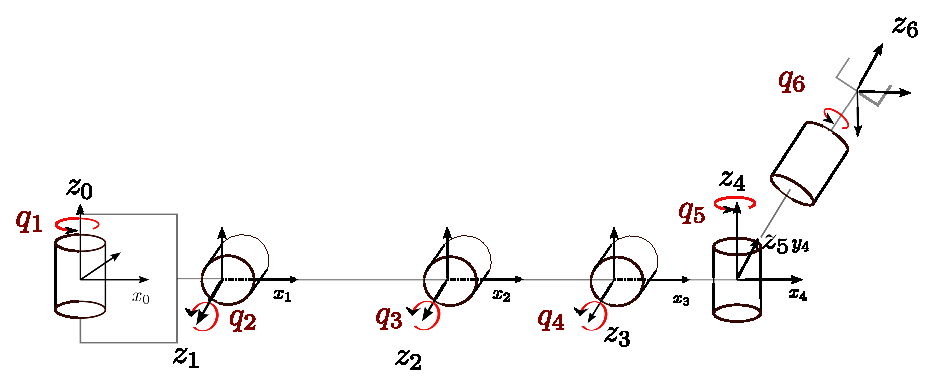
\includegraphics[scale=0.7]{./figures/manipulator_kinematics.eps}
	\caption{The frames are assigned to the kinematic structure of the manipulator according to the DH convention}
	\label{fig:dh-manipulator}
\end{figure}
For representing the orientation of the vehichle euler angles are used, which gives a minimal representation of the attitude at the expense of giving representational singulatities, see e.g. \cite{fs}. The position is represented as the coordinates of the origin of $\mathcal{F}_b$ relative to $\mathcal{F}_0$. The configuration of the manipulator are represented using the angles $q$. The total configuration given in generalized coordinates can then be written in vector form.
\begin{align*}
  \xib&:= \left[ \etab^T \bs q^T \right]^T \in \mathbb{R}^{6+n}
  \\
  \etab &= \begin{bmatrix}\etab_1 \\ \etab_2 \end{bmatrix}  = \begin{bmatrix} x_{0b} \\ y_{0b} \\ z_{0b} \\ \phi \\ \theta \\ \psi \end{bmatrix} \in \mathbb{R}^{6}
\end{align*}
One of the challenges to UVM systems is the mix of euclidean and non euclidean transformations representing the configuration of the system. While the transformation of each link is euclidean, the transformation of the vehicle is non-Euclidean \footnote{see i.e. \cite{kristin_jant} for a detailed discussion} , and in general the following is true
\begin{align}
	\bs \omega_{0b} \neq & \etadotb_2
  \label{eq:quasi1}
\end{align}
We will therefor use quasi-velosities $ \zetab $ or $\zetab^S$ to represent the velocity state of the system
\begin{align}
  \zetab &= \begin{bmatrix} \vbb \\ \qdot \end{bmatrix}
  \label{eq:zeta1}
	\\
	\zetab^S &= \begin{bmatrix} \vb{0b}{S} \\ \qdot \end{bmatrix}
	\label{eq:zetas}
\end{align}
Where $\vbb = \begin{bmatrix} \bs v^{T} & ( \bs \omega_{0b}  )^{T} \end{bmatrix}=  \begin{bmatrix} u & v & w & p & q & r \end{bmatrix}^T \in \mathbb{R}^6 $ is the body velocity twist, and $\zetab^S$ is the corresponding Spatial velocities as defined in \cite{kristin_jant}. The quasi coordinates can be mapped to the time derivative of the generalized coordinates through, \cite{kristin_jant} 
\begin{align}
 	\xidotb &=\bs J_a(\etab_2)\zetab 
  \label{eq:quasi_trans}
  \\
  \bs J_a &= \begin{bmatrix} \bs R_{0b}(\eta_2) & 0& 0 \\ 0 & \bs T_{0b}(\eta_2) & 0 \\ 0 & 0 & I \end{bmatrix} \in \mathbb{R}^{(6+n) \times (6+n) }
  \label{eq:jacobian_a}
\end{align}
Where $\bs T_{0b}(\eta_2)$ is written as in \cite{fs}.
\begin{align}
	\dot{\bs \eta}_2 & = \bs T\left( \bs \eta_{2} \right) \bs \omega_{0b}^{b} \\
	\bs T\left( \bs \eta_{2} \right) &= 
		\begin{bmatrix} 1 & s\phi t\theta & c\phi t\theta \\
										0 & c\phi & -s\phi \\
										0 & \frac{s\phi}{c\theta} & \frac{c\phi}{c\theta}
	\end{bmatrix}
	\label{eeq:fossen-transfomrm}
\end{align}
Where $s \; \cdot = sin(\cdot ), \; c \; \cdot = cos(\cdot)$ and $t \; \cdot = tan(\cdot)$. Throughout the paper several velocity variables will be used, so it is appropriate with a definition


\begin{mdframed}[style=graybox]
\begin{align}
&	\vb{0e}{B}\; - \; \text{Velocity of the end effector frame \frame e relative to \frame 0 as seen from \frame e} \nonumber
\\
& \vb{0b}{B}\; - \; \text{Velocity of \frame b relative to \frame 0 as seen from the vehicle frame \frame b} \nonumber
\\
&	\vb{0e}{S}\; - \; \text{Velocity of \frame e relative to \frame 0 in spatial coordinates relative to \frame 0} \nonumber
\\
&	\vb{0b}{S}\; - \; \text{Velocity of \frame b relative to \frame 0 in spatial coordinates relative to \frame 0} \nonumber
\end{align}

\end{mdframed}



Using the notation from \cite{kristin_jant} we define the body joint twist of a revolute joint as 
\begin{align}
	\bs X_i^i&=\begin{bmatrix} 0&0&0&0&0&1\end{bmatrix}^T
	\label{eq:body_twist}
\end{align}
It should be noted that the twist only has one nonzero component in the angular motion around the z axis due to following the Denavit-Hartenberg (DH) convention. It should also be noted that the body joint twist represents the direction of allowed motion seen from the body of link i, and is therefor always constant.
Next we define the spatial joint twist of a revolute joint as the allowed motion of each link relative to the frame $\mathcal{F}_0$, as written in \cite{kristin_jant}
\begin{align}
	\bs X_i&=\adg{0i}\bs X_i^i
	\label{eq:spatioal_twist}
\end{align}
Where the adjoint map between two frames \frame a and \frame b is defined as
\begin{align}
	\adg{ab}  &= \begin{bmatrix} \bs R_{ab} & \widehat{\bs p}_{ab}\bs R_{ab} \\ \bs 0 & \bs R_{ab} \end{bmatrix}
	\label{eq:adjoint}
  \\
	\adg{ab}^{-1} &= \begin{bmatrix} \rb{ab}^T & - \rb{ab}^T \widehat{\bs p}_{ab} \\ 0 & \rb{ab}^T \end{bmatrix}
	\label{eq:adjoint2}
\end{align}
Where \rb{ab} is the rotation matrix from \frame{a} to \frame{b}, and \pb{ab} is the vector representing the linear displacement of the origo of \frame b wrt. to \frame a. It should be noted that \adg{ab} can be seen as a map from body velocity \vb{ab}{B} to spatial velocity \vb{ab}{S}.
The hat operator $\widehat{(\cdot)}$ maps a vector to it's skew symmetric matrix representation, and when operating on a vector $\bs \omega \in \mathcal{R}^3$ is defined as
 \begin{align}
   \widehat{\bs \omega}&= \begin{bmatrix} 0 & -\omega_3 & \omega_2 \\ \omega_3 & 0 & -\omega_1 \\ -\omega_2 & \omega_1 & 0 \end{bmatrix} 
   \label{eq:skewsym}
 \end{align}
Using  \eqref{eq:adjoint} and \eqref{eq:body_twist} we get

\begin{align}
	\bs X_i&=\begin{bmatrix}\rb{0i} & \widehat{\bs p}_{0i} \rb{0i} \\ \bs 0 & \rb{0i}^T \end{bmatrix}\bs X_i^i
	\label{eq:adjoint_calc}
	\\
	&= \left[\begin{smallmatrix}{}r_{11} & r_{12} & r_{13} & p_{2} r_{31} - p_{3} r_{21} & p_{2} r_{32} - p_{3} r_{22} & p_{2} r_{33} - p_{3} r_{23}\\r_{21} & r_{22} & r_{23} & - p_{1} r_{31} + p_{3} r_{11} & - p_{1} r_{32} + p_{3} r_{12} & - p_{1} r_{33} + p_{3} r_{13}\\r_{31} & r_{32} & r_{33} & p_{1} r_{21} + p_{2} r_{11} & p_{1} r_{22} + p_{2} r_{12} & p_{1} r_{23} + p_{2} r_{13}\\0 & 0 & 0 & r_{11} & r_{12} & r_{13}\\0 & 0 & 0 & r_{21} & r_{22} & r_{23}\\0 & 0 & 0 & r_{31} & r_{32} & r_{33}\end{smallmatrix}\right]
	\left[  \begin{smallmatrix}0\\0\\0\\0\\0\\1 \end{smallmatrix}  \right]
	\\
	&=\left[\begin{smallmatrix}{}p_{2} r_{33} - p_{3} r_{23}\\- p_{1} r_{33} + p_{3} r_{13}\\p_{1} r_{23} + p_{2} r_{13}\\r_{13}\\r_{23}\\r_{33}\end{smallmatrix}\right]
\end{align}
Next we want to find a map from the generalized and quasi velocities to the velocities of each frame $\mathcal{F}_i$ with respect to the inertial frame \frame 0 in spatial coordinates. We also note the mapping between spatial and body velocities
\begin{align}
	\bs V_{0i}^S &=  \adg{0i} \bs V_{0i}^B  
  \label{eq:adg0b1}
 \end{align}
Following the notation in \cite{kristin_jant} we write the mapping from the velocities $\zetab$ to the velocities of frame $\mathcal{F}_i$ in both spatial and body coordinates
\begin{align}
	\vb{0i}{S}&= \jb{gi}{S}(\xib)\zetab^S
  \label{eq:spatial_jacobi}
  \\
	\jb{gi}{S}(\xib) &= \begin{bmatrix} \adg{0b} & \adg{0b} \bs J_i\end{bmatrix}
  \label{eq:spatial_jacobi2}
	\\
	\vb{0i}{B}&= \jb{gi}{B}(\xib)\zetab
  \label{eq:body_jacobi}
  \\
	\jb{gi}{B}(\xib) &= \begin{bmatrix} \adg{bi}^{-1} & \adg{bi}^{-1} \bs J_i\end{bmatrix}
  \label{eq:body_jacobi2}
\end{align}
Where $\bs J_i$ is the spatial geometric Jacobian of link i as written in \cite{kristin_jant} mapping the joint velocities to the spatial twist of link $i$
\begin{align}
  \bs V_{bi}^S &=\bs J_i(q)\dot q
  \label{eq:mappint1}
	\\
	\bs J_i&=\begin{bmatrix}  \bs X_1 & \bs X_2 & \cdots & \bs X_i & \bs 0_{6 \times (n-i)}    \end{bmatrix}
	\label{eq:Ji}
\end{align}
From \eqref{eq:spatial_jacobi} and \eqref{eq:body_jacobi} we get that the end effector velocity can be described using the following
\begin{align}
	\vb{0e}{S} &= \jb{ge}{S}\zetab^S
	\label{eq:ee_velo}
	\\
	&=\begin{bmatrix} \adg{0b} & \adg{0b}\jb{n}{}\end{bmatrix}\zetab^S
	\\
	\vb{0e}{B} &= \jb{ge}{B}\zetab
	\label{eq:ee_velo_body}
	\\
	&= \begin{bmatrix} \adg{bi}^{-1} & \adg{bi}^{-1} \bs J_n\end{bmatrix}\zetab
\end{align}
Where \jb{n}{} is defined in \eqref{eq:Ji} with $i=n$. We can now summarize the velocity kinematics
\begin{mdframed}[style=graybox]
	\begin{align}
	\vb{0i}{S}&=\jb{gi}{S}\zeta^S \\
	\vb{0e}{S}&=\jb{ge}{S}\zeta^S \\
	\zetab^S&=\begin{bmatrix} (\vb{0b}{S})^T & (\qdot)^T \end{bmatrix}^T \\
	\zetab^B&=\begin{bmatrix} (\vb{0b}{B})^T & (\qdot)^T \end{bmatrix}^T \\
	\vb{0i}{S}&=\adg{0i}\vb{0i}{B}
\end{align}
\end{mdframed}
%dynamics

\subsection{Dynamics}
The dynamics of the UVMS describes the motion of the vehicle in terms of forces, pose, velocities, and acceleration. The mathematical models describing the motion can be described through Newtons law of motion $F=ma$. As customary in modelling of ship dynamics and robotics, the equations of motion is derived from the knowledge of the total energy of the system using the Lagrangian $L$
\begin{align}
	L=T-V
	\label{eq:lagrange}
\end{align}
Where $T$ and $V$ is the kinetic and potential energy, respectively. Due to the high number of states of the system, the equations of motion are presented in a matrix form, adopted from the robotics litterature, which also has been customary in modern litterature on marine craft modeling and control. First, the equation of motion of the sole vehicle is presented, before the total system, including the manipulator is described.

\subsubsection{Vehicle Dynamics}

A model of a marine craft is proposed in \cite{fs} 

% fossens equations
\begin{align}
\bs M_{RB}\dot{\bs V}_{0b}^B + \bs C_{RB}(\bs V_{0b}^B)\bs V_{0b}^B + \bs g(\bs \eta) + \bs g_0 + \bs M_A \dot{\bs V}_{r}^B  + \bs C_A(\bs V_{r}^B) \bs V_{r}^B + \bs D(\bs V_{r}^B)\bs V_{r}^B = \bs \tau + \bs \tau_{wind} + \bs \tau_{wave} 
\label{eq:fossen1}
\end{align}
Where $ \bs V_{r}^B = \bs V_{0b}^B - \bs V_c^{B}$ is the velocity of the vehichle relative to the water surrounding it, and $ \bs V_{c}^{B}$ is the irrotational current as observed from $\mathcal F_b$. Using the equation in \cite{fs} with a slight change of notation, the equation of the current yields

\begin{align}
	\bs V_c^{B}&=\begin{bmatrix} u_c & v_c & w_c & 0 & 0 & 0\end{bmatrix}^T 
  \label{eq:current}
  \\
  &= \begin{bmatrix} \bs v_c^b & 0 & 0 & 0 \end{bmatrix}^T
  \\
  \bs v_c^0 &= \bs R_{0b}\bs v_c^b 
	\label{eq:current-rotation}
  \\
  \dot{\bs v}_c^i&=0
\end{align}
Where $v_{c}^{0}$ is the constant linear current as observed in the inertial frame \frame 0. It should be noted that since the rotation matrix in \eqref{eq:current-rotation} in general is time varying, the current velocity as observed in the body frame is also time varying. 

Using the properties of an irrational constant current \cite{fs} 
\begin{align}
  \bs C_{RB}(\bs V_{r}^B) &= \bs C_{RB}(\bs V_{0b}^B) 
  \label{eq:irrational}\\
\end{align}
The equation of motion can be written as 
\begin{align}
  \bs M \dot{\bs V}_r + \bs C(\bs V_{r}^B)\bs V_r + \bs D(\bs V_{r}^B)\bs V_{r}^B +  \bs g(\bs \eta) + \bs g_0  &= \bs \tau + \bs \tau_{wind} + \bs \tau_{wave} 
  \label{eq:fossen2}\\
  \bs M &= \bs M_{RB} + \bs M_A
  \label{eq:massCol} \\
  \bs C(\bs V_r^B) &= \bs C_{RB}(\bs V_r^B)+ \bs C_A(\bs V_r^B)
\end{align}


% full UVMS dynamics
\subsubsection{Vehicle Manipulator Dynamics}
The dynamics for the veichle can be included in the total dynamics of the UVMS. As the operation of the UVMS is modelled as being totally submerged, the wind will be removed from \eqref{eq:fossen2}, and the force from waves will be neglected, which is reasonable since the operation will mostly take place in sufficiently deep waters.

Each link of the manipulator can be modelled as a rigid body according to \eqref{eq:fossen2} but looking at the coupled dynamics of the rigid bodies the inertia matrix $\bs M$ is no longer constant but varies with the configuration $\bs q$. The generalized coordinates and generalised and quasi velocities can be written in two separate variables

\begin{align}
  \xib  & := \left[ \bs \eta^T \bs q^T \right]^T
  \label{eq:xi} \\
  \zetab & := \left[ (\vbb)^T \qdot^T \right]^T
  \label{eq:zeta}
\end{align}
and the dynamics of the total system is written in \cite{antonelli1} as

\begin{align}
  \bs M(q)\zetadotb + \bs C(q,\zetab) \bs \zeta +\bs D(q,\zetab) + \bs N(\xib)=\taub
  \label{eq:antonelliDynamics}
\end{align}
where $\bs N(\xib)$ is the gravitational and boyancy forces acting on the vehicle and manipulator. In \eqref{eq:antonelliDynamics} the current is not included in the dynamics, and the author proposes a model in the same form as \eqref{eq:fossen1} with separated rigid body and hydrodynamic terms:

\begin{align}
  \bs M_{RB}\zetadotb+ \bs C_{RB}(\zetab)\zetab + \bs g(\bs \eta) + \bs g_0 + \bs M_A \zetadotb_r  + \bs C_A(\zetab_r) \zetab_r + \bs D(\zetab_r) \zetab_r = \bs \tau 
  \label{eq:withinteraction}
\end{align}
Where $\zetab_r = \begin{bmatrix} (\bs V_r^B)^T & \qdot^T  \end{bmatrix}^T$ is velocity of the system relative to the current. Note that it is sufficient that the vector $\zetab_r$ includes only the relative motion of the vehicle, since the kinematic chain of the manipulator moves relative to the vehichle. Since the current is irrotational and constant the contribution of the linear velocity of the vehicle adds the hydrodynamic terms caused by the current. 

Since the UVMS uses the end effetor to interact with the environment, it is important to include the generalized forces due to contact between the end effector and the environment. Using \cite{spong2005robot} we get the contribution from the interaction forces projected on the generalized forces using the geometric Jacobian $\bs J_{ge}^B$ through the relationship

\begin{align}
  \bs \tau&= (\bs J_{ge}^B)^T \bs F 
  \label{eq:jacobian_force}
\end{align}
Where $\bs F= [f_x, f_y, f_z, n_x, n_y,n_z]^T  $ is the vector of forces and moments from the environment to the end effector. We can then include the interaction forces to the total dynamics

\begin{mdframed}[style=graybox]
\begin{align}
  \bs M_{RB}\zetadotb+ \bs C_{RB}(\zetab)\zetab + \bs g(\bs \eta) + \bs g_0 + \bs M_A \zetadotb_r  + \bs C_A(\zetab_r) \zetab_r + \bs D(\zetab_r) \zetab_r =\bs \tau+ (\bs J_{ge}^B)^T \bs F 
\label{eq:dyn_with_current}
\end{align}
\end{mdframed}



























